\chapter{Results}
\label{chap:Four}

\section{Experiment setting and Model Architecture}
\label{sec:expset}

\subsection{Application Experiment Setting}
\label{subsec:tool}
To test the performance of our data anonymization and our application generally, we needed to get the largest amount of real world users we can get. We managed to reach an agreement with the team teaching CSEN 603 which is the Software Engineering course in the GUC led by Dr.Aysha Alsafty
to publish the application for the students enrolled in this course. In this course students are divided into groups of 10 and try to develop the best web-application for real clients.
We encouraged teams to post pictures and text posts while they were working on their projects and to further incentivize students to participate we also stated that there would be an award
for the most active team in the awards ceremony held at the end of semester.
We also stated that all data collected will be deleted at the end of project and will be used only for the purposes of this research strictly to address their privacy concerns.
\subsection{ML Model Architecture}
\label{subsec:data}
For the models we decided to use Keras\cite{chollet2015keras} which is a model-level library, providing high-level building blocks for developing deep learning models. Keras offers simple APIs for the users which makes it easy to learn and use espically for simple models.
It also provides 3 backend enginges for to choose from TensorFlow/Theano/CNTK for the purposes of this research we decided to choose TensorFlow as it is widely adopted and has the highest support availability incase we encountered any problems.
The models we built are fairly simple relative to other deep neural network models as the the relations weren't complex in both of the datasets.\par

The classifier for the first dataset consisted of 2 hidden dense layers each having 4 nodes, both of the hidden layers used “RELU” as their activation function and used L2-Regularization to improve the loss function, the output layer was placed after the 2 hidden layers and had only 1 node with a sigmoid activation function. We configured to model to use “Binray Crossentropy” as the loss function as
we are trying to classify whether 2 students are friends or not.
\begin{figure}[H]
  \centering
  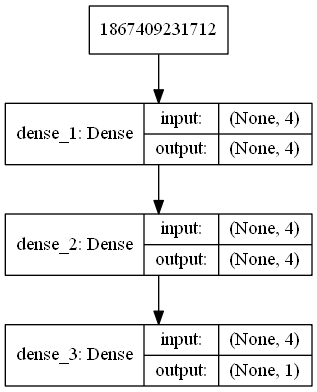
\includegraphics[scale=0.65]{model}
  \caption{Model 1 Diagram}
  \label{fig:Model1}
\end{figure}
As for the second Model this one was more complex as we first had to use one hot encoding (OHE) to encode all room locations,date/timeSlot fields and student's names as well which were all generated in text form which can't be fed to the Model directly.
What OHE does simply is that it counts the number of unique values in a column and then creates new columns equal to the numbers of these unique values in the column where every new column corresponds to 1 of the unique values, The new columns are filled by checking which unique value was present for this row and put a “1” in it's corresponding newly generated column and “0”s in all other generated columns while the rest of the data for the row is unchanged.
For this model we had to do multiple tweaks to the architecture of the model as we progressed with the data obfuscation however these details will be discussed thoroughly in the next chapter and we will only state the baseline architecture of the model in this section,
The model consisted of 3 layers, The first layer is the input layer which had a dimensionality of 184 due to using OHE on the rows while the second layer is the only hidden layer which had 20 nodes and used a “RELU” activation function and also used L2-Regularization to minimize the loss function and prevent overfitting, finally the last
layer which is the output layer consisted of 38 nodes which represented 38 unique room locations and used “Softmax” as it's activation function.\par
\begin{figure}[H]
    \centering
    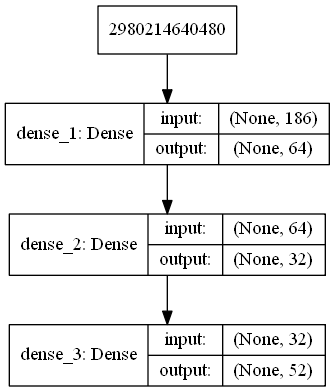
\includegraphics[scale=0.65]{model3}
    \caption{Model 2 Baseline Diagram}
    \label{fig:Model2}
  \end{figure}
The 2 models used “Adam” as their optimizer as it can handle gradients with big differences which our dataset maybe suffering from, in addition to being able to handle noisy data and very easy to configure and use



\section{Application Experiment Results}
\label{sec:expres}
Evaluating the effectiveness of an experiment involving a mobile application generally involves measuring the time performance of different aspects of the backend of the application, performing analysis on the application's users and finally analyze the collected data through the application.
\subsection{Application Users}
\label{subsec:Application}
We managed to get 46 registerd user on our backend who consumed about 1.6GB of bandwidth of our 10GB Quota for downloads/uploads during a 2 month duration and 50MB out of a 1GB Quota of consistent storage on our fireback database, however about 5 of those were accounts made for testing the application throughout the semester thus the number of real world users is about 40.
In this section we will be performing statistical analysis on various aspects of the user's profiles such as users gender distribution which was used to get more accurate reccomendations for users, users choices of privacy and the results we got from the questionnaire that was provided inside the application after registration.\par

Regarding the gender distribution we offered 3 options being (Male,Female,Private) for each registering user, the statistics at the time of writing this excluding the test users was as follows,
we had 20 Male users, 14 Female users, and 6 users who refused to specify their gender. We note that the low number of users who refused to share their gender shows that either most users don't see a risk by sharing their gender or they trust our application to share it.
It is also noted that the higher number of Male users shows that Male users are more likely try out new applications to help with their testing especially that our testing was done in the Computer Science department where student might have an intrest to tryout new applications.
\begin{figure}[H]
    \centering
    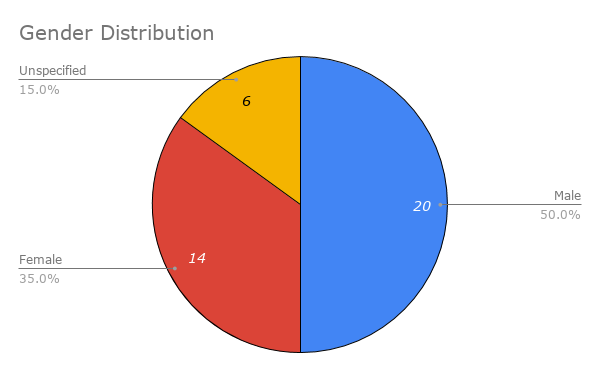
\includegraphics[scale=0.55]{Gender}
    \caption{User's Gender Distribution}
    \label{fig:Gender}
\end{figure}

As for the Privacy level chosen by the users, we also offered 3 levels of privacy as mentioned in [\ref{Part:PrivacyLev}]. The privacy distribution was found to be as follows, The highest chosen setting was the medium privacy setting with 17 users choosing it followed by the high privacy setting chosen by 13 users and finally the lowest privacy setting was selected by 10 which was more than excepted.
In the next chapter we will discuss these findings and numbers and what we can conclude from these values and what they mean to us and their correlation with other values.
\newline
\newline
\begin{figure}[H]
    \centering
    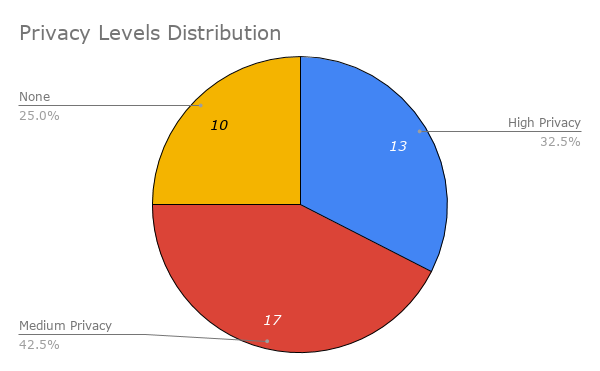
\includegraphics[scale=0.55]{PrivacyChart}
    \caption{User's Privacy Level Distribution}
    \label{fig:PrivacyLevels}
\end{figure}

Now moving onto the data collected from the application, our application was used in collecting data of various forms, images, text, and ratings. In total we had 103 data points distributed as follows, 67 Image Posts, 22 Text posts and 14 Image ratings.
\begin{figure}[H]
    \centering
    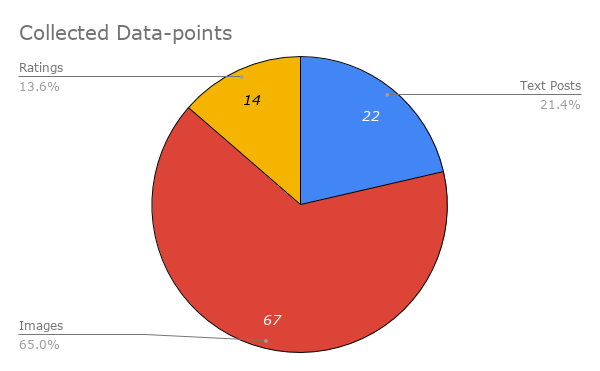
\includegraphics[scale=0.55]{Data-points}
    \caption{Submitted Data Distribution}
    \label{fig:DataPoints}
\end{figure}
\subsection{Application Backend Performance}
In this section we will discuss how long it takes for Images/Text to be posted to the backend, what features of faces the face detection algorithm can detect, how different modes of face detection behave and blur and how long it takes to blur these faces,
how long it takes to load user's timeline and finally how much time it takes for the registration/login process.
\newline
\newline
\newline
\newline
The following timings were recorded using Moment.js which is the most popular date/time manipulation library in Javascript.
Login and registration are pretty fast, however to get an accurate timinig and mitigate any network issues we tested each operation 5 times and got the average. It is also noted that the amount of data transfered when logging-in or registering is minimal so network speed will not be a factor in this benchmarking process.
The average time for logging in was \num{4488.1}ms while the average time for registering was \num{5374.1}ms which is 12\% higher since logging in is just matching a record with no POST request while the registeration we perform validation checks on the front-end and on the backend.
As for the loading the data from the backend database this is excepted to have the largest time and worst performance since we currently don't perform any data chunking and load all submitted Images/Text posts regardless of date submitted or if it is seen before whenever a user views his Timeline.
The average time for loading the data was \num{14795.4}ms. We state the exact value for each trial in the table below.
\begin{table}[!h]
    \addtolength{\tabcolsep}{-4pt}
    \begin{tabular}{|l|l|l|l|l|l|l|}
    \hline
    \textbf{} & \textbf{1st} & \textbf{2} & \textbf{3} & \textbf{4} & \textbf{5} & \textbf{Average Time(ms)} \\ \hline
    \textbf{Login} & \textbf{3553} & \textbf{2820.1} & \textbf{8210} & \textbf{4240} & \textbf{3621} & \textbf{4488.1} \\ \hline
    \textbf{Register} & \textbf{5879.45} & \textbf{6092.38} & \textbf{5455.367} & \textbf{4727.55} & \textbf{4718.8} & \textbf{5374.1} \\ \hline
    \textbf{LoadTimeline} & \textbf{15089} & \textbf{15463} & \textbf{14446} & \textbf{14793} & \textbf{14186} & \textbf{14795.4} \\ \hline
    \end{tabular}
    \caption{Average Loading Time for backend operations}
    \label{tab:my-table}
\end{table}



Now moving onto the face detection algorithm and blurring algorithm, the face detection model that firebase provided had 2 modes, a fast mode and an accurate mode, here we detail the functional differences between each of them.\par
For both the “ACCURATE” mode and the “FAST” mode the maximum number of faces we could detect was 6 faces in 1 image however, the “ACCURATE” mode provided more powerful detection features such as being able to detect partially obscured faces behind other objects
as well as being to detect faces that have been rotated to the right or to the left relative to the device's camera in contrast to the “FAST” mode where the detected faces can only be rotated upwards or downards, however this trade-off comes at the cost of the detection speed. The full pipeline in the “FAST” mode takes \num{6579}ms to detect up to 6 faces in 1 image and blur them incase a high privacy level is chosen and save it to the database
while the “ACCURATE” mode pipeline takes up to \num{14747.02} ms to process the same image. We repeat the time measuring process used above in the following table by averaging the time measured for uploading and blurring the same image 5 times.
\newline
\begin{table}[!h]
    \addtolength{\tabcolsep}{-2.75pt}
    \begin{tabular}{|l|l|l|l|l|l|l|}
    \hline
    \textbf{} & \textbf{1} & \textbf{2} & \textbf{3} & \textbf{4} & \textbf{5} & \textbf{Average Time(ms)} \\ \hline
    \textbf{FAST} & \textbf{7092.1} & \textbf{6395.7} & \textbf{6524.4} & \textbf{6440.1} & \textbf{6444.5} & \textbf{6579.36} \\ \hline
    \textbf{ACCURATE} & \textbf{14782} & \textbf{14931.5} & \textbf{14798.7} & \textbf{14501.9} & \textbf{14720.8} & \textbf{14747.02} \\ \hline
    \end{tabular}
    \caption{Average Time for FAST and ACCURATE modes}
    \label{tab:FASTACC}
\end{table}

The “ACCURATE” mode also offers facial features detection such as smile detection, face countor detection however these features weren't useful for our purpose so we won't be going into their details.
\section{ML Models Results}
In this section we will be evaluating the results of the 2 models we outlined earlier using the datasets generated in [\ref{chap:Three}] however we will be applying tweaks to these datasets to simulate applying incremental privacy and consequently we will have some tweaks to the second model architecture to improve it's performance in response to incremental privacy.\par
All the models described below were trained locally on a machine with the following hardware specifications CPU: Intel I5-4460 GPU: Nvidia GTX 1060 6GB RAM: 16GB
\subsection{Friendship Prediction Model}
This model is a very simple model to predict as it doesn't have any complex features or relations moreover, the predicted value is generated by a function that we invented which is pretty easy for a (ANN) to learn and approximate.
We split the dataset into an 80-20 training and validation split and started training using the model stated in [\ref{fig:Model1}] and started the training process with 50 epochs however we noticed that the model was overfitting heavily where we managed to get a training accuracy of 100\%, We later discovered that this was caused due to 2 reasons first, high number of epochs compared to the dataset size as we had a high number of steps per epoch which caused our model to see the same data multiple times and secondly, our dataset as it suffered from a data-leak.
A dataleak is when the training data contains the prediction that the model should learn, In our case we included the value of the friendship function which determined whether 2 students should be friends or not, to solve this we removed this column from the training and validation data and reduced the number of the epochs to 30 while keep the same steps per epoch.
\begin{figure}[H]
    \centering
    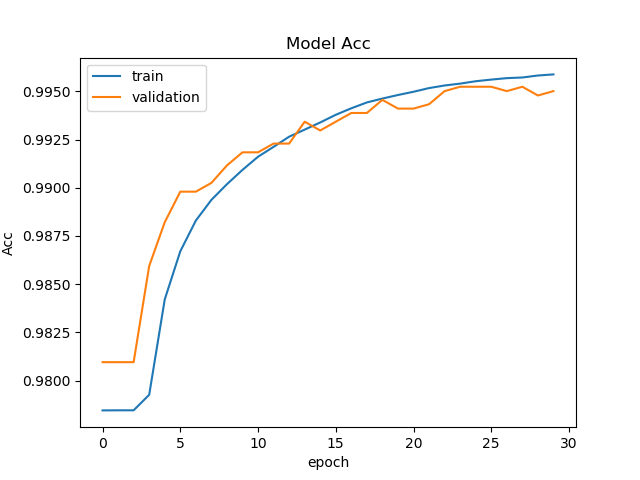
\includegraphics[scale=1]{FriendMod}
    \caption{Training and validation accuracy}
    \label{fig:ResultFriends}
\end{figure}
Looking at this curve it is noted that at some points the validation accuracy is higer than the testing accuracy this is caused due to following, Every Keras model has 2 operation modes, Training and Testing, in the training mode Regularization mechanisms such L1/L2 regularization and drop-out are used however,
when Keras switches the model to testing mode all regularization mechanisms are turned off moreover, the reported training loss is actually the average of the losses over batches of training data and losses at the first epochs is generally higher than losses at later ones. On the other hand, the testing loss which is computed at the end of an epoch using the model as it is without considering previous batches thus, resulting in a lower loss.
The above can also be verified by making the model predict the labels for the training and testing data after it is done trainig we can see it the trainig accuracy is actually higher.
It is also noted that the fluctuations in both the training and validation accuracy are very small fluctuations in the range of 0.0020 however they may appear otherwise due to plotting the labels with 4 decimal places. 
\begin{figure}[H]
    \centering
    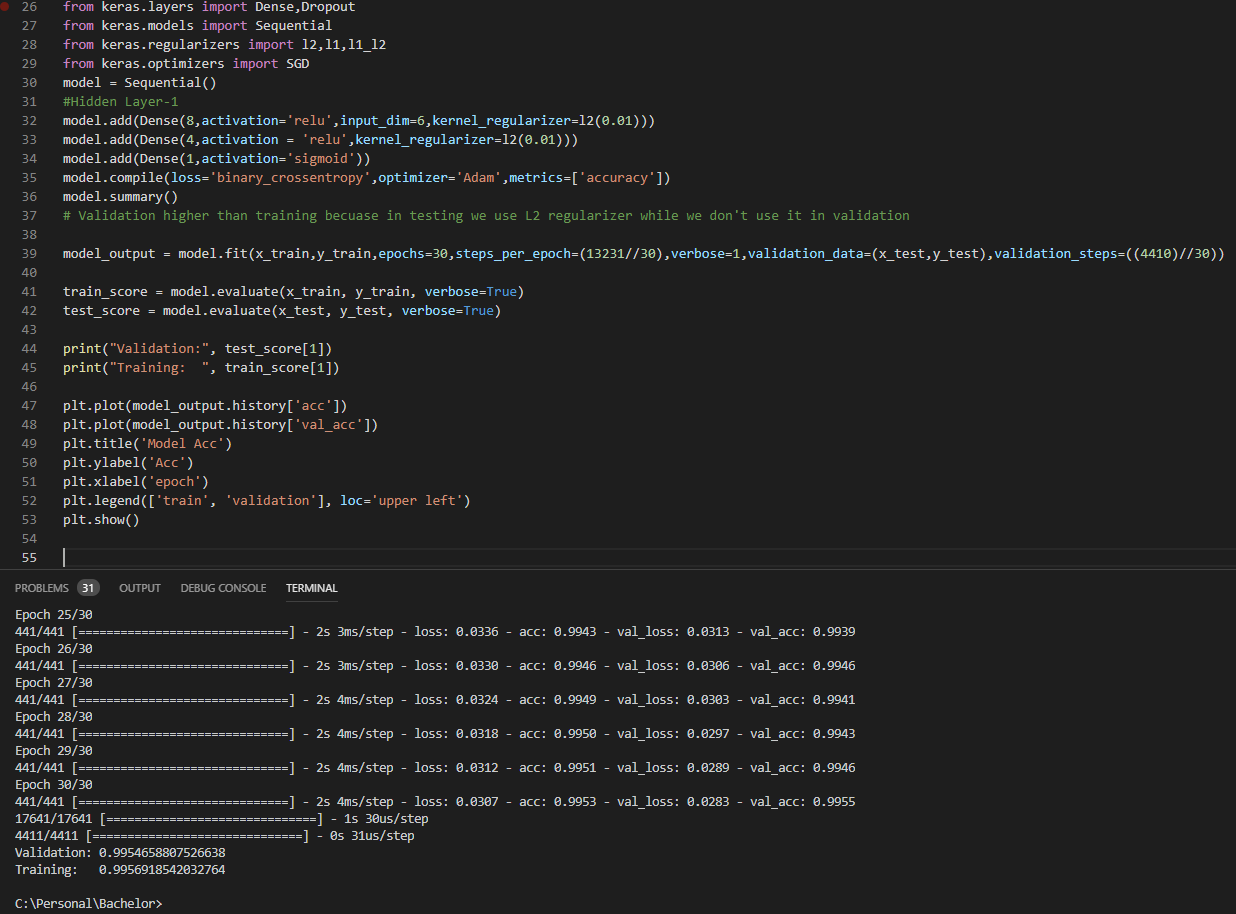
\includegraphics[scale=0.55]{Verification}
    \caption{Verification of [\ref{fig:ResultFriends}]}
    \label{fig:Verification}
\end{figure}

We decided not to simulate any kind of incremental privacy for this model as this dataset was just created to see if we are on the right track and to help us in creating the second model which is our original goal

\subsection{GUC Location Prediction Model}
